\documentclass[aspectratio=169,13pt,t] {beamer}
%
% Choose how your presentation looks.
%
% For more themes, color themes and font themes, see:
% http://deic.uab.es/~iblanes/beamer_gallery/index_by_theme.html
%
\mode<presentation>
{
  \usetheme{Madrid}      % or try Darmstadt, Madrid, Warsaw, ...
  \usecolortheme{beaver} % or try albatross, beaver, crane, ...
  \usefonttheme{serif}  % or try serif, structurebold, ...
%  \setbeamertemplate{navigation symbols}{}
  \setbeamertemplate{caption}[numbered]
  \setbeamertemplate{items}[default]
}

\usepackage[,UTF8,linespread=1.2]{ctex}
\usepackage{wrapfig}
\usepackage{caption}
\captionsetup[figure]{name=图,labelsep=period}
\usepackage[,most]{tcolorbox}
\usepackage{picinpar}


\usepackage{xcolor}
\definecolor{xy_blue}{cmyk}{0.6,0.35,0.0,0.4}
\definecolor{xy_orange}{cmyk}{0.0,0.7,1.0,0.0}
\definecolor{xy_green}{cmyk}{0.2,0.0,1.0,0.15}
\xdefinecolor{xy_gold}{RGB}{135,103,79}
\xdefinecolor{xy2_gold}{cmyk}{0,0.35,0.75,0.05}


\setbeamercolor{section number projected}{fg=red,bg=red!20}%控制球的颜色
\setbeamercolor{subsection number projected}{fg=blue,bg=blue!40}
\setbeamercolor{item}{fg=xy_gold} %设置列表项颜色

\usepackage{amsthm}
\newtheorem{peroration}{结论：}
\newtheorem{exploration}{探究：}
\newtheorem{prooft}{证明：}
\newtheorem{question}{问题}
\newtheorem*{solve}{解:}
\newtheorem{instance}{例}   % 解：独立计数器
\BeforeBeginEnvironment{peroration}{%
	\setbeamercolor{block title}{bg=xy_green,fg=white}
	\setbeamercolor{block body}{bg=xy_green!10}
}
\AfterEndEnvironment{peroration}{
	\setbeamercolor{block title}{bg=xy_blue,fg=white}
	\setbeamercolor{block body}{bg=xy_blue!10}
}
\BeforeBeginEnvironment{exploration}{%
	\setbeamercolor{block title}{bg=xy_orange,fg=white}
	\setbeamercolor{block body}{bg=xy_orange!10}
}
\AfterEndEnvironment{peroration}{
	\setbeamercolor{block title}{bg=xy_blue,fg=white}
	\setbeamercolor{block body}{bg=xy_blue!10}
}
\BeforeBeginEnvironment{solution}{%
	\setbeamercolor{block title}{bg=xy_green,fg=white}
	\setbeamercolor{block body}{bg=xy_green!10}
}
\AfterEndEnvironment{solution}{
	\setbeamercolor{block title}{bg=xy_green,fg=white}
	\setbeamercolor{block body}{bg=xy_green!10}
}
\BeforeBeginEnvironment{prooft}{%
	\setbeamercolor{block title}{bg=xy_green,fg=white}
	\setbeamercolor{block body}{bg=xy_green!10}
}
\AfterEndEnvironment{prooft}{
	\setbeamercolor{block title}{bg=xy_green,fg=white}
	\setbeamercolor{block body}{bg=xy_green!10}
}
\BeforeBeginEnvironment{question}{%
	\setbeamercolor{block title}{bg=xy_orange,fg=white}
	\setbeamercolor{block body}{bg=xy_orange!10}
}
\AfterEndEnvironment{question}{
	\setbeamercolor{block title}{bg=xy_green,fg=white}
	\setbeamercolor{block body}{bg=xy_green!10}
}
\BeforeBeginEnvironment{solve}{%解：
	\begingroup
	\setbeamercolor{block title}{bg=xy_orange!60,fg=white}
	\setbeamercolor{block body}{bg=xy_orange!10}
}
\AfterEndEnvironment{solve}{%解：
	\endgroup
}

\setbeamercolor{prooft}{fg=red, bg=green!10}       % 标题颜色
\setbeamercolor{prooft body}{fg=red, bg=red!5}  % 内容块背景
\setbeamerfont{prooft head}{series=\bfseries}       % 标题字体
\setbeamerfont{question body}{shape=\upshape}         % 内容字体
\renewcommand{\thefigure}{\arabic{figure}}

\newtcolorbox{summarybox}[1][]{
	colback=purple!10,
	colframe=purple!70!black,
	fonttitle=\bfseries,
	title=#1,
	arc=1mm,
	boxrule=0pt,drop shadow,
	left=2mm, right=2mm, top=2mm, bottom=2mm,
}
\newtcolorbox{summarybox-answer}{
	width=0.9\textwidth,
	colback=white,
	blanker,
	borderline west={2pt}{20pt}{cyan},
	left=10mm, right=2mm, top=2mm, bottom=2mm,
	}
\title[4.2指数函数]{4.2\ 指数函数}
\subtitle{指数函数的概念、图象和性质}
\author[好好学习，努力向上]{}
\institute{}
\date{2026.10.13}
%\setbeamertemplate{theorems}[numbered]
\theoremstyle{definition}
\newtheorem{exam}{例}
\AtBeginSection[]
{
  \begin{frame}<beamer>
    \frametitle{本节主要内容}
    \tableofcontents[currentsection,currentsubsection]
  \end{frame}
}

\AtBeginDocument{
	\setlength{\abovedisplayskip}{3pt}
	\setlength{\belowdisplayskip}{3pt}
	\setbeamertemplate{theorems}[numbered]
}

\usepackage{pgfplots}
\pgfplotsset{compat=1.18}
\usetikzlibrary{arrows.meta}

\begin{document}
\begin{frame}{}
	\titlepage
\end{frame}

\begin{frame}{内容概览}
	\tableofcontents
\end{frame}

\section{指数函数的概念}

\begin{frame}{问题引入：景区游客人次}
	自 2001 年起，A、B 两地景区采取了不同的应对措施：A 地提高门票价格，B 地取消门票. 以 2001 年游客人次为 \(y\) 倍，经过 \(x\) 年：
	\begin{itemize}
		\item A 景区游客人次近似\textbf{线性增长}，年增加量大致相等（约 10 万次）；
		\item B 景区游客人次近似\textbf{指数增长}，每年游客人次约为上一年的 \(1.11\) 倍.
	\end{itemize}
	\vspace{1em}
	\pause
	于是 B 景区游客人次可近似描述为：
	\[
		y=1.11^x\quad (x\in[0,+\infty)).
	\]
	这里指数 \(x\) 是自变量，底数 \(1.11\) 是一个大于 \(0\) 且不等于 \(1\) 的常量.
\end{frame}

\begin{frame}{问题引入：碳 14 的衰减}
	生物死亡后，体内碳 14 含量按确定比率衰减，大约每经过 \(5\,730\) 年衰减为原来的一半（\textbf{半衰期}）.
	\vspace{0.5em}
	设死亡生物体内碳 14 含量为 \(y\)，死亡年数为 \(x\)，则
	\[
		y=\left(\left(\frac12\right)^{\frac{1}{5730}}\right)^x\quad (x\in[0,+\infty)).
	\]
	\vspace{1em}
	\pause
	\begin{summarybox-answer}
		无论是指数增长 \(y=1.11^x\)，还是指数衰减 \(y=\left(\left(\frac12\right)^{\frac{1}{5730}}\right)^x\)，它们都具有共同的结构：指数是自变量，底数是一个大于 \(0\) 且不等于 \(1\) 的常量.
	\end{summarybox-answer}
\end{frame}

\begin{frame}{指数函数的定义}
	\begin{summarybox}[指数函数（exponential function）]
		一般地，函数
		\[
			\boxed{\,y=a^x\quad (a>0,\ \text{且}\ a\neq 1)\,}
		\]
		叫做\textbf{指数函数}，其中指数 \(x\) 是自变量，定义域是 \(\mathbf{R}\).
	\end{summarybox}
	\vspace{1em}
	\pause
	\begin{summarybox-answer}
		\textbf{思考：}为什么规定 \(a>0\) 且 \(a\neq 1\)？\\
		若 \(a\leqslant 0\)，则某些 \(x\) 时 \(a^x\) 无意义；若 \(a=1\)，则 \(1^x\equiv 1\)，是常数函数，没有研究价值.
	\end{summarybox-answer}
\end{frame}

\begin{frame}{例1：求函数值}
	\begin{exam}
		已知指数函数 \(f(x)=a^x\)（\(a>0\)，且 \(a\neq 1\)），且 \(f(3)=\pi\)，求 \(f(0)\)，\(f(1)\)，\(f(-3)\) 的值.
	\end{exam}
	\pause
	\begin{solve}
		因为 \(f(x)=a^x\)，且 \(f(3)=\pi\)，则 \(a^3=\pi\)，解得 \(a=\pi^{\frac{1}{3}}\)，于是
		\[
			f(x)=\pi^{\frac{x}{3}}.
		\]
		所以
		\[
			f(0)=\pi^0=1,\quad f(1)=\pi^{\frac{1}{3}}=\sqrt[3]{\pi},\quad f(-3)=\pi^{-1}=\frac{1}{\pi}.
		\]
	\end{solve}
\end{frame}

\begin{frame}{指数增长模型 \(y=k a^x\)}
	在实际问题中，经常遇到类似于指数增长的指数模型：设原有量为 \(N\)，每次的增长率为 \(p\)，经过 \(x\) 次增长，该量增长到 \(y\)，则
	\[
		y=N(1+p)^x\quad (x\in \mathbf{N}).
	\]
	\vspace{1em}
	\begin{summarybox-answer}
		形如 \(y=k a^x\)（\(k\in \mathbf{R}\)，\(k\neq 0\)；\(a>0\)，且 \(a\neq 1\)）的函数是刻画\textbf{指数增长}或\textbf{指数衰减}变化规律的非常有用的函数模型.
	\end{summarybox-answer}
\end{frame}

\section{指数函数的图象和性质}

\begin{frame}{画出 \(y=2^x\) 的图象}
	先从最简单的函数 \(y=2^x\) 开始. 列出 \(x,y\) 的对应值表，用描点法画出图象：
	\vspace{0.5em}
	\begin{center}
		\small
		\begin{tabular}{|c|c|c|c|c|c|c|c|c|}
			\hline
			\(x\) & \(-2\) & \(-1.5\) & \(-1\) & \(-0.5\) & \(0\) & \(0.5\) & \(1\) & \(2\) \\ \hline
			\(y=2^x\) & \(0.25\) & \(0.35\) & \(0.5\) & \(0.71\) & \(1\) & \(1.41\) & \(2\) & \(4\) \\ \hline
		\end{tabular}
	\end{center}
	\vspace{0.5em}
	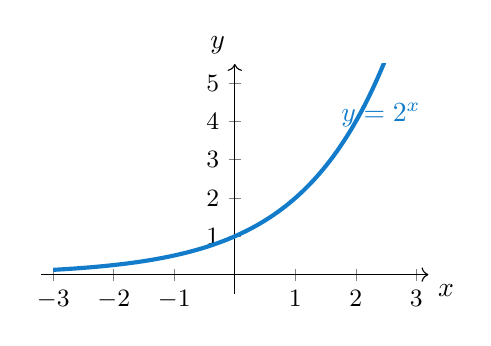
\begin{tikzpicture}[baseline=(current bounding box.center)]
		\begin{axis}[
			width=6.5cm, height=4.5cm,
			xmin=-3.2, xmax=3.2,
			ymin=-0.5, ymax=5.5,
			xtick={-3,-2,-1,0,1,2,3},
			ytick={1,2,3,4,5},
			axis lines=middle,
			axis line style={->},
			xlabel={$x$}, ylabel={$y$},
			xlabel style={below right},
			ylabel style={above left},
			tick label style={font=\small},
		]
		\addplot[color=cyan!60!blue, line width=1.5pt, domain=-3:2.6, samples=100] {exp(x*ln(2))};
		\node[above right, cyan!60!blue] at (1.6, 3.6) {$y=2^x$};
		\end{axis}
	\end{tikzpicture}
\end{frame}

\begin{frame}{\(y=\left(\frac12\right)^x\) 与对称性}
	\begin{summarybox}[探究]
		画出函数 \(y=\left(\frac12\right)^x\) 的图象，并与函数 \(y=2^x\) 的图象进行比较，它们有什么关系？
	\end{summarybox}
	\vspace{0.5em}
	因为 \(y=\left(\frac12\right)^x=2^{-x}\)，点 \((x,y)\) 与点 \((-x,y)\) 关于 \(y\) 轴对称，所以函数 \(y=2^x\) 图象上任意一点 \(P(x,y)\) 关于 \(y\) 轴的对称点 \(P_1(-x,y)\) 都在函数 \(y=\left(\frac12\right)^x\) 的图象上.
	\vspace{0.5em}
	\begin{summarybox-answer}
		底数互为倒数的两个指数函数的图象关于 \(y\) 轴对称.
	\end{summarybox-answer}
\end{frame}

\begin{frame}{对比图象：\(y=2^x\) 与 \(y=\left(\frac12\right)^x\)}
	\begin{center}
	\begin{tikzpicture}
		\begin{axis}[
			width=9cm, height=6.5cm,
			xmin=-3.5, xmax=3.5,
			ymin=-0.5, ymax=5.5,
			xtick={-3,-2,-1,0,1,2,3},
			ytick={1,2,3,4,5},
			axis lines=middle,
			axis line style={->},
			xlabel={$x$}, ylabel={$y$},
			xlabel style={below right},
			ylabel style={above left},
			tick label style={font=\small},
			legend pos=north west,
			legend style={font=\small},
		]
		\addplot[color=cyan!60!blue, line width=1.5pt, domain=-3:2.6, samples=100] {exp(x*ln(2))};
		\addlegendentry{$y=2^x\ (a>1)$}
		\addplot[color=pink!70!purple, line width=1.5pt, domain=-2.6:3, samples=100] {exp(-x*ln(2))};
		\addlegendentry{$y=(\tfrac12)^x\ (0<a<1)$}
		\addplot[only marks, mark=*, mark size=2pt, color=black] coordinates {(0,1)};
		\node[below right] at (0,1) {$(0,1)$};
		\end{axis}
	\end{tikzpicture}
	\end{center}
\end{frame}

\begin{frame}{底数 \(a\) 的两类图象}
	选取底数 \(a\) 的若干个不同值，在同一直角坐标系内画出相应的指数函数图象，可以发现图象按底数 \(a\) 的取值分为 \(0<a<1\) 和 \(a>1\) 两种类型.
	\vspace{0.5em}
	\begin{center}
	\begin{tikzpicture}
		\begin{axis}[
			width=8.5cm, height=5.5cm,
			xmin=-3, xmax=3,
			ymin=-0.5, ymax=5.5,
			xtick={-2,-1,0,1,2},
			ytick={1,2,3,4,5},
			axis lines=middle,
			axis line style={->},
			xlabel={$x$}, ylabel={$y$},
			xlabel style={below right},
			ylabel style={above left},
			tick label style={font=\small},
		]
		\addplot[color=cyan!60!blue, line width=1.2pt, domain=-2.6:2.3, samples=80] {exp(x*ln(2))};
		\addplot[color=blue!60!black, line width=1.2pt, domain=-2.6:1.8, samples=80] {exp(x*ln(3))};
		\addplot[color=pink!70!purple, line width=1.2pt, domain=-2.3:2.6, samples=80] {exp(-x*ln(2))};
		\addplot[color=red!60!black, line width=1.2pt, domain=-1.8:2.6, samples=80] {exp(-x*ln(3))};
		\node[above right, cyan!60!blue] at (1.7, 3.2) {$y=2^x$};
		\node[above left, pink!70!purple] at (-1.9, 3.2) {$y=(\tfrac12)^x$};
		\end{axis}
	\end{tikzpicture}
	\end{center}
\end{frame}

\begin{frame}{指数函数的性质}
	\begin{center}
	\renewcommand{\arraystretch}{1.4}
	\begin{tabular}{|c|c|c|}
		\hline
		& \(0<a<1\) & \(a>1\) \\ \hline
		\textbf{图象} & 过 \((0,1)\) 下降 & 过 \((0,1)\) 上升 \\ \hline
		\textbf{定义域} & \multicolumn{2}{|c|}{\(\mathbf{R}\)} \\ \hline
		\textbf{值域} & \multicolumn{2}{|c|}{\((0,+\infty)\)} \\ \hline
		\textbf{定点} & \multicolumn{2}{|c|}{过定点 \((0,1)\)，即 \(x=0\) 时 \(y=1\)} \\ \hline
		\textbf{单调性} & \textbf{减函数} & \textbf{增函数} \\ \hline
	\end{tabular}
	\end{center}
	\vspace{1em}
	\pause
	\begin{summarybox-answer}
		当 \(a>1\) 时，\(x>0\) 则 \(y>1\)，\(x<0\) 则 \(0<y<1\)；当 \(0<a<1\) 时相反.
	\end{summarybox-answer}
\end{frame}

\begin{frame}{例3：比较两个值的大小}
	\begin{exam}
		比较下列各题中两个值的大小：
		\begin{enumerate}[(1)]
			\item \(1.7^{2.5}\)，\(1.7^{3}\)；
			\item \(0.8^{-\sqrt{2}}\)，\(0.8^{-\sqrt{3}}\)；
			\item \(1.7^{0.3}\)，\(0.9^{3.1}\).
		\end{enumerate}
	\end{exam}
\end{frame}

\begin{frame}{例3 解答}
	\begin{solve}
		\begin{enumerate}[(1)]
			\item \(1.7^{2.5}\) 与 \(1.7^{3}\) 可看作函数 \(y=1.7^x\) 当 \(x\) 分别取 \(2.5,3\) 的函数值. 因为 \(1.7>1\)，\(y=1.7^x\) 是增函数，且 \(2.5<3\)，所以 \(1.7^{2.5}<1.7^{3}\).
			\item 因为 \(0<0.8<1\)，\(y=0.8^x\) 是减函数. 因为 \(-\sqrt{2}>-\sqrt{3}\)，所以 \(0.8^{-\sqrt{2}}<0.8^{-\sqrt{3}}\).
			\item 由指数函数性质：\(1.7^{0.3}>1.7^0=1\)，\(0.9^{3.1}<0.9^0=1\)，所以 \(1.7^{0.3}>0.9^{3.1}\).
		\end{enumerate}
	\end{solve}
\end{frame}

\begin{frame}{例4：城市人口的指数增长}
	\begin{exam}
		如图，某城市人口呈指数增长.
		\begin{enumerate}[(1)]
			\item 根据图象，估计该城市人口每翻一番所需的时间（倍增期）；
			\item 该城市人口从 \(80\) 万人开始，经过 \(20\) 年会增长到多少万人？
		\end{enumerate}
	\end{exam}
	\pause
	\begin{solve}
		\begin{enumerate}[(1)]
			\item 观察图象，该城市人口经过 \(20\) 年约为 \(10\) 万人，经过 \(40\) 年约为 \(20\) 万人，即由 \(10\) 万人增加到 \(20\) 万人所用时间约 \(20\) 年，所以人口每翻一番所需时间约 \(20\) 年.
			\item 因为倍增期为 \(20\) 年，每经过 \(20\) 年人口翻一番. 从 \(80\) 万人开始，经过 \(20\) 年，人口大约会增长到 \(160\) 万人.
		\end{enumerate}
	\end{solve}
\end{frame}

\section{课堂练习}

\begin{frame}{练习 1：判断指数函数图象}
	\begin{question}
		下列图象中，有可能表示指数函数的是（\quad ）.
		\begin{enumerate}[(A)]
			\item 一条下降直线
			\item 开口向上的抛物线
			\item 从左下向右上上升、且在 \(x\) 轴上方的曲线
			\item 过原点、穿过一、三象限的曲线
		\end{enumerate}
	\end{question}
	\pause
	\begin{solve}
		指数函数 \(y=a^x\) 的图象都在 \(x\) 轴上方（值域为 \((0,+\infty)\)），过定点 \((0,1)\)，且是\textbf{曲线}而非直线. 故选 \textbf{(C)}.
	\end{solve}
\end{frame}

\begin{frame}{练习 2：求指数函数解析式}
	\begin{question}
		已知函数 \(y=f(x)\)，\(x\in \mathbf{R}\)，且 \(f(0)=3\)，\(\dfrac{f(0.5)}{f(0)}=2\)，\(\dfrac{f(1)}{f(0.5)}=2\)，\(\cdots\)，\(\dfrac{f(0.5n)}{f(0.5(n-1))}=2\)，\(n\in \mathbf{N}^{*}\)，求函数 \(y=f(x)\) 的一个解析式.
	\end{question}
	\pause
	\begin{solve}
		由 \(\dfrac{f(0.5(n))}{f(0.5(n-1))}=2\) 知，自变量每增加 \(0.5\)，函数值乘 \(2\)，即底数 \(a^{0.5}=2\)，所以 \(a=4\). 又 \(f(0)=3\)，故
		\[
			f(x)=3\cdot 4^x.
		\]
	\end{solve}
\end{frame}

\begin{frame}{练习 3：比较大小}
	\begin{question}
		比较下列各题中两个值的大小：
		\begin{enumerate}[(1)]
			\item \(3^{0.8}\)，\(3^{0.7}\)；
			\item \(0.75^{-0.1}\)，\(0.75^{0.1}\)；
			\item \(1.01^{2.7}\)，\(1.01^{3.5}\).
		\end{enumerate}
	\end{question}
	\pause
	\begin{solve}
		\begin{enumerate}[(1)]
			\item \(3>1\)，\(y=3^x\) 增函数，\(0.8>0.7\)，所以 \(3^{0.8}>3^{0.7}\)；
			\item \(0<0.75<1\)，\(y=0.75^x\) 减函数，\(-0.1<0.1\)，所以 \(0.75^{-0.1}>0.75^{0.1}\)；
			\item \(1.01>1\)，\(y=1.01^x\) 增函数，\(2.7<3.5\)，所以 \(1.01^{2.7}<1.01^{3.5}\).
		\end{enumerate}
	\end{solve}
\end{frame}

\begin{frame}{布置作业}
	\begin{summarybox}[课后作业]
		\begin{enumerate}
			\item 教材 P119 习题 4.2：复习巩固 1，2，3
			\item 教材 P119 习题 4.2：综合运用 6，7
			\item 预习：4.3.1 对数的概念
		\end{enumerate}
	\end{summarybox}
\end{frame}

\end{document}
